%%%%%%%%%%%%%%%%%%%%%%%%%%%%%%%%%%%%%%%%%%%%%%%%%%%%%%%%%%%%%%%%%%%%%%%%%%%%
% AGUtmpl.tex: this template file is for articles formatted with LaTeX2e,
% Modified July 2014
%
% This template includes commands and instructions
% given in the order necessary to produce a final output that will
% satisfy AGU requirements.
%
% PLEASE DO NOT USE YOUR OWN MACROS
% DO NOT USE \newcommand, \renewcommand, or \def.
%
% FOR FIGURES, DO NOT USE \psfrag or \subfigure.
%
%%%%%%%%%%%%%%%%%%%%%%%%%%%%%%%%%%%%%%%%%%%%%%%%%%%%%%%%%%%%%%%%%%%%%%%%%%%%
%
% All questions should be e-mailed to latex@agu.org.
%
%%%%%%%%%%%%%%%%%%%%%%%%%%%%%%%%%%%%%%%%%%%%%%%%%%%%%%%%%%%%%%%%%%%%%%%%%%%%
%
% Step 1: Set the \documentclass
%
% There are two options for article format: two column (default)
% and draft.
%
% PLEASE USE THE DRAFT OPTION TO SUBMIT YOUR PAPERS.
% The draft option produces double spaced output.
%
% Choose the journal abbreviation for the journal you are
% submitting to:

% jgrga JOURNAL OF GEOPHYSICAL RESEARCH
% gbc   GLOBAL BIOCHEMICAL CYCLES
% grl   GEOPHYSICAL RESEARCH LETTERS
% pal   PALEOCEANOGRAPHY
% ras   RADIO SCIENCE
% rog   REVIEWS OF GEOPHYSICS
% tec   TECTONICS
% wrr   WATER RESOURCES RESEARCH
% gc    GEOCHEMISTRY, GEOPHYSICS, GEOSYSTEMS
% sw    SPACE WEATHER
% ms    JAMES
% ef    EARTH'S FUTURE
% ea    EARTH AND SPACE SCIENCE
%
%
%
% (If you are submitting to a journal other than jgrga,
% substitute the initials of the journal for "jgrga" below.)

\documentclass[grl]{agutex}   %draft, [ms]
% To create numbered lines:

% If you don't already have lineno.sty, you can download it from
% http://www.ctan.org/tex-archive/macros/latex/contrib/ednotes/
% (or search the internet for lineno.sty ctan), available at TeX Archive Network (CTAN).
% Take care that you always use the latest version.

% To activate the commands, uncomment \usepackage{lineno}
% and \linenumbers*[1]command, below:

\usepackage{lineno}
\linenumbers*[1]
%  To add line numbers to lines with equations:
%  \begin{linenomath*}
%  \begin{equation}
%  \end{equation}
%  \end{linenomath*}
%%%%%%%%%%%%%%%%%%%%%%%%%%%%%%%%%%%%%%%%%%%%%%%%%%%%%%%%%%%%%%%%%%%%%%%%%
\usepackage{url}
\usepackage{amsmath}
\usepackage{rotating} 

\usepackage{lineno}
\usepackage[bottom]{footmisc}

\usepackage{graphics}

%\usepackage[dvips]{graphicx}
 
\usepackage{color}
\definecolor{pinkred}{rgb}{1.0, 0.4, 0.4}

% Author names in capital letters:
\authorrunninghead{HUANG ET AL.}

% Shorter version of title entered in capital letters:
\titlerunninghead{}

%Corresponding author mailing address and e-mail address:
\authoraddr{Corresponding author: Xingying Huang,
Department of Land, Air and Water Resources, \\
 University of California Davis, Davis, CA 95616, USA.
 (xyhuang@ucdavis.edu)}
 
%Department of Hydrology and Water Resources, University of
%Arizona, Harshbarger Building 11, Tucson, AZ 85721, USA.
%(a.b.smith@hwr.arizona.edu)}

\begin{document}

%% ------------------------------------------------------------------------ %%
%
%  TITLE
%
%% ------------------------------------------------------------------------ %%


\title{}
%
% e.g., \title{Terrestrial ring current:
% Origin, formation, and decay $\alpha\beta\Gamma\Delta$}
%

%% ------------------------------------------------------------------------ %%
%
%  AUTHORS AND AFFILIATIONS
%
%% ------------------------------------------------------------------------ %%

%Use \author{\altaffilmark{}} and \altaffiltext{}

% \altaffilmark will produce footnote;
% matching \altaffiltext will appear at bottom of page.

% \authors{A. B. Smith,\altaffilmark{1}
% Eric Brown,\altaffilmark{1,2} Rick Williams,\altaffilmark{3}
% John B. McDougall\altaffilmark{4}, and S. Visconti\altaffilmark{5}}

%\altaffiltext{1}{Department of Hydrology and Water Resources,
%University of Arizona, Tucson, Arizona, USA.}

%\altaffiltext{2}{Department of Geography, Ohio State University,
%Columbus, Ohio, USA.}

%\altaffiltext{3}{Department of Space Sciences, University of
%Michigan, Ann Arbor, Michigan, USA.}

%\altaffiltext{4}{Division of Hydrologic Sciences, Desert Research
%Institute, Reno, Nevada, USA.}

    \authors{Xingying Huang,\altaffilmark{1}
  Paul A. Ullrich, \altaffilmark{1} }

\altaffiltext{1}{Department of Land, Air and Water Resources, University of California, Davis}


%%%%%%%%%%%%%%%%%%%%%%%%%%%%%%%%%%%%%%%%%%%%%%%%%%%%%%%%%%%%%%%%%%%%%
% ABSTRACT
%
% Enter your Abstract here

\begin{abstract}

\end{abstract}

\begin{article}


%%%%%%%%%%%%%%%%%%%%%%%%%%%%%%%%%%%%%%%%%%%%%%%%%%%%%%%%%%%%%%%%%%%%%
% MAIN BODY OF PAPER
%%%%%%%%%%%%%%%%%%%%%%%%%%%%%%%%%%%%%%%%%%%%%%%%%%%%%%%%%%%%%%%%%%%%%
%
\section{Introduction}

Over past decades, human behaviors have strongly impacted the climate both globally and regionally mostly with increasing greenhouse gases(citation). Another important factor is land cover changes such as deforestation and urbanization \citep{bonan1997effects, pielke2002influence, kueppers2008seasonal, diffenbaugh2009influence}. Due to the expansion of the human population, conversion of natural land surface to cropland is prominent. What affects the climate is not only the cropland itself but also the human activities imposed on it. Harvest affects regional climate obviously through albedo changes, and net radiation changes including both sensible and latent heat fluxes (foley2003green, add citation). Additionally, the land management also plays a important role in affecting the climate by modifying the carbon and water cycles such as different length of cropping and irrigation (lobell2006biogeophysical, add citation). 


%In some areas with extensive irrigation, the cooling effect by irrigation can match or even exceed the impacts of greenhouse warming [Diffenbaugh, 2009; Kueppers et al., 2007; Lobell et al., 2008; Puma and Cook, 2010].


Previous studies showed that (irrigation cooling effect (add studies here)) with increasing latent heat and ground evaporation. The effect of irrigation on climate seems to be much more prominent than the land surface change (govindasamy2001land, bounoua2002effects, matthews2004natural add citation). California is the topmost irrigating State in the U.S., and most of the irrigated cropland is at California's Central Valley (CV), with its vast agricultural industry and in contrast the extremely dry growing seasons of the Mediterranean climate. CV ranges nearly 600 km from north to south, and 60-100 km from west to east. The CV produce 25$\%$ of the agricultural products in the United States, and about (?km3, (30 km3/yr? doll2002global)) of water each year is used over 52,000 km$^2$ of irrigated area \citep{famiglietti2011satellites}. irrigated area (shiklomanov2000appraisal, siebert2005development, add citation). (bonfils2007empirical) found that irrigation over CV has decreased summertime maximum temperature by $\sim$2-3 K in heavily-irrigated areas compared with nearby non-irrigated areas, from long-term temperature records. (add more studies)

%irrigated water and area for year 2000 http://pubs.usgs.gov/circ/2004/circ1268/htdocs/table07.html  http://pubs.usgs.gov/circ/2004/circ1268/htdocs/text-ir.html

%More than half of this area (CV) has been converted to agriculture since the presettlement period. The Central Valley produces one quarter of the agricultural products in the United States, with an annual income exceeding $26 billion and an export revenue exceeding $6.7 billion (Wilkinson et al. 2002). Thus, understanding the climate variability in this area is critical for projecting future economic sustainability in California and the USA. It accounts for one sixth of the country�s irrigated land [Faunt, 2009].

%bonfils2007empirical found that irrigation expansion has had a large cooling effect on summertime average daily daytime temperatures (0.14�C to 0.25�C per decade), which corresponds to an estimated cooling of 1.8�C to 3.2�C since the introduction of irrigation practices. Irrigation has negligible effects on nighttime temperatures, leading to a net cooling effect of irrigation on climate (0.06�C to 0.19�C per decade). Stabilization of irrigated area has occurred in California since 1980 and is expected in the near future for many irrigated regions. 

%Mahmood et al. (2006) found an irrigation-induced cooling of *1 K in maximum growing season temperatures in irrigated areas in Nebraska.
%The cooling was much stronger for daily maximum than minimum temperatures, decreasing the diurnal temperature range.

%may compare the VR-CESM ensemble run 1 and nrrig run to see the land cover change effect over CV
%"the resulting increase in atmospheric water vapor may also enhance cloud cover and downstream precipitation." what is downstream precipitation?
%check: snyder2006regional
%Irrigation has been used on over 35 000 km2 in California alone (USDA 2007).

%lobell2008effect

For more info of irrigation over CA, see table 1, 2, 6, 7 in \citep{canessa2011agricultural} Agricultural Water Use in California: A 2011 Update

Influences of irrigation are often ignored in climate modeling due to multiple reasons including its small area ($\sim$2$\%$ of global land surface) and its seeming negligible cooling effect compared compared with global greenhouse warming \citep{boucher2004direct}. However, with the increasing need for regional climate studies, irrigation practice could be a important factor regulating heavy irrigated area's climate patterns. For this purpose, climatic effects of irrigation have been modeled mainly by limited-area models (LAMs) (or referred as regional climate models (RCMs)) (kueppers2007irrigation, add citation). For example, \citet{adegoke2003impact} found reduced near-surface temperature over irrigated land in Nebraska, with the fraction of irrigation grid cells is set up to be saturated at 0000 UTC each day. (xx found that xx). Irrigation was modeled differently among those studies including when the irrigation is needed, how much irrigated water will be added, and the area of cropland that will be irrigated. Therefore, the magnitude of the irrigation cooling effect is not only related with the specific land surface model but also controlled by the way irrigation works. Though global climate models (GCMs) are rarely used to account for irrigation effect, it is also important to find out how the climate changes when adding irrigation into GCMs. \citet{lobell2006biogeophysical} coupled the community atmosphere model (CAM, add version here) to the community land model (CLM, add version here) to model irrigation by fixing soil moisture at saturation during the growing season in all croplands. And the results showed that irrigation caused a global land surface cooling of 1.3 K, and regional cooling of up to 8 K. \citet{sacks2009effects} also used the CAM (add version here) coupled to the CLM (add version here) and compared global simulations with and without irrigation, and found that irrigation alters climate significantly in some regions with cooling effect of near surface temperature for about 0.5 K averaged over the year. \citet{lo2013irrigation} used the CAM 3.5 combined with the CLM 3.5 at $\sim$1.4$^\circ$, and showed that the increase in evapotranspiration and water vapor due to irrigation significantly impacts the atmospheric circulation in the southwestern United States with a anthropogenic loop in the regional hydrological cycle.


%sacks2009effects: "The cooling effect of irrigation seemed to be dominated by indirect effects like an increase in cloud cover, rather than by direct evaporative cooling. The regional effects of irrigation were as large as those seen in previous studies of land cover change, showing that changes in land management can be as important as changes in land cover in terms of their climatic effects. Our results were sensitive to the area of irrigation, but were insensitive to the details of irrigation timing and delivery." why cloud cover???

%The irrigation effects could potentially enhance shallow and deep convections and increase cloud formation [Kawase et al., 2008; Qian et al., 2013] and precipitation [DeAngelis et al., 2010; Koster et al., 2004; Segal et al., 1998] by modifying the depths of planetary boundary layer, lifting condensation level, and mixing layer.

%Kueppers et al. (2007) investigated the irrigation cooling effect over California. They found that the conversion of natural vegetation to irrigated crops has cooled irrigated areas by *3.7 K in August and *1.6 K yearround. Averaged over all of California, they found that irrigation (along with other land cover changes) has decreased August temperatures by *0.4 K. Kueppers et al. (2007), in contrast, performed their irrigation by holding root zone soil moisture fixed at field capacity year-round in irrigated grid cells. They did not report how much water they added through irrigation, an omission common to many irrigation modeling studies. Using RegCM3, Kueppers et al. [2007] simulated the effect of irrigation on regional climate in the Central Valley, California, at interannual scales of irrigation, they forced the RegCM3 root zone (top 1 m) soil moisture to field capacity at every time step during the simulation period. (30km)

%Recently, climate research groups in California have conducted a model intercomparison study of the climate response to land-use change in the western United States (Kueppers et al. 2008; hereafter referred to as K08). All of the models showed large decreases in August mean and maximum 2-m air temperatures where irrigation replaced natural vegetation. Kueppers et al. [2008] compared the effects of irrigation on regional climate, with specific emphasis on summer temperatures. Based on simulations by the different Regional ClimateModels (RCMs), they found that the behavior of RCMs varied, depending on each model�s physics, as well as on irrigation configurations.

%Mahmood et al. (2004, 2006) found a decreasing trend in daily maximum temperature under irrigated land use in Nebraska.
%Weare and Du (2008) explored the influences of global warming and land use changes on past climate change in California and conclude that in summer, irrigation has a strong effect on the differences between recent and past conditions in maximum temperature, surface latent and sensible heat fluxes, surface moisture, and surface humidity.

%sorooshian2011significant got that simulation results with fine model resolution and with the more realistic irrigation scheme indicate that the surface meteorological fields are noticeably improved when compared with observations from the CIMIS network and Moderate Resolution Imaging Spectroradiometer data. Our results also indicate that irrigation has significant impacts on local meteorological fields by decreasing temperature by 3��7�C and increasing relative humidity by 9�20%, depending on model resolutions and allowable soil water depletion configurations. More significantly, our results using the improved model show that the effects of irrigation on weather and climate do not extend very far into nonirrigated regions.

%"Many studies have quantitatively investigated the impact of irrigation on weather, climate, and hydrology at different scales. Such studies have relied mainly on the use of physics-based numerical models"

Though previous studies as aforementioned have worked on the irrigation effect over California, they either used RCMs or GCMs at coarse resolution (check out the degree of lobell2006, $\sim$2.8$^\circ$ for sacks2009effects) with differences of irrigation magnitude and coverage. ("In fact, how much water should be added into soil is still unresolved and depend on models"). In order to model regional climate over CV, relatively fine horizontal resolution is needed for a more accurate representation of microclimates, land-use, small-scale dynamical features and interactions and to provide more useful info for formulating climate adaptation and mitigation strategies \citep{leung2003regional, rauscher2010resolution}. In this paper, we use the recently developed variable-resolution Community Earth System Model (VR-CESM) as our GCM to study the impact of irrigation on regional climate over CV in California, combined with realistic estimates of regional agricultural water use as described in Section 2. VRGCM uses a relatively coarse global model with enhanced resolution over a specific region \citep{staniforth1978variable, fox1997finite}. Compared with RCMs, a key advantage of VRGCMs is that they use a single, unified modeling framework, rather than separate GCM and RCM with potentially disparate dynamics and physics parameterizations. Compared to uniform-resolution global models, VRGCMs provide a cost-effective method of reaching high resolutions over a region of interest -- the limited area simulations in this study at $28$ km resolution represent a reduction in required computation of approximately 10 times. VRGCMs have been demonstrated to be effective for regional climate studies and applications at a reduced computational cost compared to uniform GCMs (zarzycki2015effects, Rhoades2015Characterizing, Huang2015).

%LAMs may suffer from potential inconsistencies between the global and regional scales and lack two-way interactions at the nest boundary \citep{warner1997tutorial, mcdonald2003transparent, laprise2008challenging, mesinger2013limited}, problems that can be mitigated with the use of VRGCMs. 
%\citet{zarzycki2015effects} applied VR-CESM at 0.25$^\circ$  and fount that xx. \citet{Huang2015 studied and found that} \citet{Rhoades2015Characterizing} has also assessed the use of VR-CESM for modeling mountain snowpack in the western United States and found that.

The study applied the irrigation option in CLM 4.0 coupled in CESM 1.2.0 to investigate the impact of irrigation not only on mean climatology, but also on heat extremes over recently past climate from year 1980-01-01 to 2005-12-31 in CV. (or from 1981 to 2005). This paper is organized as follows. Section 2 describes the model setup, datasets and methodology. In section 3, simulation results are provided and discussed. Key results are summarized along with further discussion in section 4.

\section{Model setup and reference datasets}

\subsection{Irrigation modeling}

The irrigation model is implemented by applying a relatively realistic amount of irrigation water based on leaf area index (LAI) and explicitly calculate the effects on the surface water and energy balance, mostly like the way stated in \citep{sacks2009effects}. The fraction area of the cropland that equipped for irrigation is from \citep{siebert2005development, siebert2007global} matching the year 2000, and is fixed over the simulation period. This is still reasonable since over 1980s�2000s, there is no net growth of irrigation area \citep{bonfils2007empirical}. "The irrigation water usage has no seasonal and interannual variation as well as being independent of crop type."

%Siebert et al. [2005] provided a GlobalMap of Irrigated Area (GMIA) representing the fraction of area equipped for irrigation around the year of 2000 with a spatial resolution of 5 arc minutes (hereafter denoted as FGMIA). They combined input data sets from various sources such as The Food and Agriculture Organization of the United Nations reports, the United Nations, Ministries of Agriculture and land use, and land cover data set from United States Geological Survey (USGS) for the year 2000. This map has been widely used in modeling [Sacks et al., 2009; Saeed et al., 2009] and observational studies [Bonfils and Lobell, 2007; Zhu et al., 2012] and has become the defacto information source for spatial distribution of global irrigated areas of the present day.

Model checks if irrigation is needed at 6 AM local time by computing the deficit between the current soil moisture content and a target soil moisture content. If irrigation is needed, the calculated deficit is the amount of water that will be added through irrigation. The target soil moisture content in each soil layer i (wtarget,i, kg m-2) is a weighted average of (1) the minimum soil moisture content that results in no water stress in that layer (wo,i, kg m-2) and (2) the soil moisture content at saturation in that layer (wsat,i, kg m-2), (as Equation showed) \citep{oleson2010technical}. The default irrigation weight factor is 0.7, which was determined empirically to give global, annual irrigation amounts that approximately match observed gross irrigation water use around the year 2000 \citep{shiklomanov2000appraisal}. This irrigation is applied at a constant rate over the following four hours. Irrigation water is applied directly to the ground surface, bypassing canopy interception. More details about the way that the irrigation works in CLM 4.0 can be found from the on-line technical descriptions \footnote{http://www.cesm.ucar.edu/models/cesm1.2/clm/}.

(equation: wtarget,i=(1?0.7)?wo,i+0.7?wsat,i)

%(i.e., total water withdrawals for irrigation: ~ 2500 � 3000 km3 year-1 (Shiklomanov, 2000)).
%historical time series of county irrigated areas from agricultural censuses and

%There are ten soil layers, with a total depth of 3.4 m (Oleson et al. 2004).

%Sack2009 "combine the most realistic aspects of Boucher et al. 2004 and lobell2006biogeophysical. To do this, we use a global irrigation map based on census data from the Food and Agricultural Organization of the United Nations (FAO) (Helkowski 2004; Foley et al. 2005). We add the irrigation water directly to the land surface and allow the land model to determine the fraction evaporated or transpired. Thus, we use a sophisticated land surface model that calculates the partitioning between evapotranspiration and runoff, and an observation-based data set of the locations and amounts of irrigation."

%http://www.cesm.ucar.edu/models/cesm1.2/clm/  Technical descriptions of the interactive crop management (CLM4CNcrop) and interactive irrigation models in version 4 of the Community Land Model

%And we also tried to adjust the amount of irrigated water to better understand how the irrigation part works in CLM4.0. 

%On the other hand, Lobell et al. [2009], using the Community Atmospheric Model (CAM3.3) and through prescribing the top 30 cm soil moisture at the irrigation grid for 90%, 50%, 40%, and 30%of soil saturation, found that the impacts of irrigation on air temperature and latent heat fluxes are �extremely insensitive� to soil moisture increases beyond 30% saturation. The results from Lobell et al. [2009] may be relevant to the land?surface model, i.e., the Community Land Model (CLM) they used.
%The same results were done by Kueppers and Snyder [2011], who also claimed that �irrigation to 50, 75, or 100% of field capacity did not result in detectably different effects on afternoon maximum temperatures in any month of the year in RegCM3,� which is coupled with BATS LSM.

a) irrigation area: see Figure 1 (irrigatedArea.pdf) \ref{fig:Figure 1}, (as what is used in \citet{kueppers2007irrigation})  almost all the cropland over CA is irrigated crop

b) irrigation water: kern County (CA): area 8140.964496 sq. mile., irrigated water 3.0 km cubic per year (year 2000), http://www.ssjid.com/district-services/agriculture-irrigation-water.htm: Irrigation season runs from approximately March 15 to October 15, depending on the weather and water supplies. 

%We assume that there are 180 days of equal irrigation, with QRRIG at 1.5mm/day (irrigated factor = 0.7), the total irrigated water will be 5.627 km^3/year, for kern County; with QRRIG at 1.5/2 mm/day (irrigated factor = 0.5), the value is about 2.8, near 3.0 km^3/year. \citep{ozdogan2010simulating}  recalculate this the mean QIRRIG for factor 0.7 is about 0.6mm/day for 365 days


\subsection{VR-CESM}

add citation here or see supplement doc
%CESM is a state-of-the-art Earth modeling framework managed by the National Center for Atmospheric Research (NCAR), consisting of coupled atmospheric, oceanic, land and sea ice models. CESM has been frequently used for modeling present and future global climate \citep{neale2010description, hurrell2013community}. The coupling infrastructure in CESM communicates the interfacial states and fluxes between each component model so that fluxes are conserved. Since we follow the Atmospheric Model Intercomparison Project (AMIP) protocols \citep{Gates1992}, only the atmosphere and land model are integrated dynamically. Here, CAM version 5 (CAM5) \citep{CAM5Tech} and the Community Land Model (CLM) version 4 \citep{CLM40Tech} are used. The SE dynamical core, which possesses attractive conservation and parallel scaling properties \citep{dennis2011cam, taylor2011conservation}, is employed along with variable-resolution grid support. The FAMIPC5 (F$\_$AMIP$\_$CAM5) compset was chosen for these simulations.

%For our study, the variable-resolution cubed-sphere grids are generated for use in CAM and CLM with the open-source software package SQuadGen \citep{ullrich2014squadgen}. The grids used are depicted in Figure \ref{fig:VR-CESM_map}. The maximum horizontal resolution on these grids is 0.25 $^\circ$ ($\sim$ 28km), with a quasi-uniform 1 $^\circ$ mesh over the remainder of the globe. In our study and in previous studies (e.g. \citet{zarzycki2015effects}), general circulation patterns (e.g. wind, pressure and precipitation) do not exhibit apparent artifacts in the variable-resolution transition region, and the design of the SE dynamical core ensures that dry air and tracer mass are conserved globally \citep{taylor2010compatible}. Simulations were performed over the time period from 1979-01-01 to 2005-12-31 (UTC) and 1979 is discarded as a spin-up period. This time period was chosen to provide an adequate sampling of annual variability, and to limit computational cost.

%Variable-resolution topography files were produced by sampling the National Geophysical Data Center (NGDC) 2-min ($\sim$ 4 km) Gridded Global Relief Dataset (ETOPO2v2) topography dataset, followed by application of a differential smoothing technique as described in \citet{zarzycki2015effects}.  

%Land surface datasets, including plant functional types, were created using the $0.5$ $^\circ$ reference datasets. Greenhouse gas (GHG) concentrations and aerosol forcing are prescribed based on historical observations. CAM and CLM tuning parameters are not modified from their default configurations. SSTs and ice coverage are supplied by the 1 $^\circ$ Hadley Centre Sea Ice and Sea Surface Temperature dataset (HadISST) \citep{hurrell2008new}. 

\subsection{Simulations}

(Explain why 0.25 degree is enough to capture the pattern of mean climatology, e.g. topo) 

(A table of all runs as Sack 2009, and explain all the runs)

For no irrig control run, we used the pft at 0.5 degree; afterward, we found that there are higher resolution land surface dataset, then we use 3min($\sim$10 km) resolution for our irrig run. And there are rarely organizable differences (the only notable pattern is (10-20$\%$) more c3 non-arctic grass, less c3 crop in some parts of CV). (The 3min land surface dataset has more realistic percentage of cropland, resulting more accurate irrigated area) 

%The 3min dataset seems better than 0.5degree vegetation file for pft type 13 (non-arctic grass) and 15 (C3 generic crop) over WUS. 
%for 3min: surfdata_AR_30_x4_simyr2000_3min_c150721.nc ; Irrig_raw_data_file_name = "mksrf_irrig_2160x4320_simyr2000.c110527.nc" (5min) ; Vegetation_type_raw_data_filename = "mksrf_landuse_rc2000_c110913.nc" (MODIS, 3min)
%for 0.5 deg: surfdata_AR_30_x4_simyr2000_c150416.nc  ; Vegetation_type_raw_data_filename = "mksrf_landuse_rc2000_c090630.nc" (0.5*0.5 MODIS)

hourly run of year 2000

\subsection{Reference datasets}

Gridded observational datasets of the highest available quality and weather stations datasets are employed (see Table \ref{tab:Datasets}). Differences between gridded observations can be due to choice of meteorological stations, interpolation techniques, elevation models and processing algorithms. Consequently, the use of multiple reference datasets is necessary to understand the underlying uncertainty in the observational data. Detailed descriptions of these datasets are as follows.

%Although these products are employed to serve as realistic proxies for assessing the model results, we acknowledge that they may be sensitive to the choice of model. 

\paragraph{UW} The UW daily gridded meteorological data is obtained from the Surface Water Modeling group at the University of Washington \citep{maurer2002long, hamlet2005production}. UW incorporates topographic corrections by forcing the long-term average precipitation to match that of the PRISM dataset. The temperature dataset is produced in a similar fashion as precipitation, but uses a simple 6.1 K/km lapse rate for topographic effect. The dataset is provided at 0.125$^\circ$ horizontal resolution covering the period 1949 to 2010.

%With a good station coverage over California [including both the U.S. Historical Climatology Network (HCN) and Cooperative network observations (COOP)], a high 1/8�  1/8� resolution and adjustment for urbanization effects, the UW data set (38) represents our best candidate to study the contribution of irrigation to temperature variations in California.

%\paragraph{Daymet} Daymet is an extremely high resolution (1 km) gridded dataset with daily outputs of total precipitation, humidity, and minimum/maximum temperature covering the years of 1980 through 2013 \citep{thornton1997generating, thornton2014daymet}. The dataset is produced using an algorithmic technique that ingests point station measurements in conjunction with a truncated Gaussian weighting filter.  Some adjustments are made to account for topography. Daymet is available through the Oak Ridge National Laboratory Distributed Active Archive Center (ORNL DAAC). 

%For applications of the radiation and humidity data please cite thornton1999improved, thornton2000simultaneous

\paragraph{PRISM} The Parameter-elevation Regressions on Independent Slopes Model (PRISM) \citep{daly2008physiographically} supports a 4 km gridded dataset obtained by taking point measurements and applying a weighted regression scheme that accounts for many factors affecting the local climatology. The datasets include total precipitation and minimum/maximum, (derived) mean temperatures and dewpoints. Monthly climatological variables are available for 1895 through 2014 from the PRISM Climate Group (Oregon State University, \url{http://prism.oregonstate.edu}, created 4 Feb 2004). Notably, PRISM is the United States Department of Agriculture's official climatological dataset.  PRISM is used as our primary reference dataset for model performance evaluation.

\paragraph{NCDC} add description of weather station datasets here
%In all cases, the stations cover well both high and low irrigated areas

%VIC dataset: monthly mean the contiguous U.S. for the period 1950 - July 2000    0.125degree  may put this to supplement
%http://research.jisao.washington.edu/data_sets/vic/
%http://www.hydro.washington.edu/Lettenmaier/Data/livneh/livneh.et.al.2013.page.html   updated data from 1915 to 2011   \citep{livneh2013long}
%http://www.esrl.noaa.gov/psd/data/gridded/data.livneh.fluxvars.html



\section{Methodology}

"Irrigation practice in California peaks in summer and is significant in spring but is rather sparse during the fall and winter seasons \citep{salas2006estimating}."

%Since heat extremes dominate during the summer season, we focus on June, July and August (JJA) for assessment of temperature.

%(no Detrend since the trend is too small) 

%supplement

\section{results}

%Irrigation: H2OSOI	volumetric soil water (vegetated landunits only)	mm3/mm3  the soil has 15 layers, but change only occurs to the first ten layers, particularly the first three layers. decide to calculate the average for 15 layers  0 to 0.05mm3/mm3 (JJA)
%QIRRIG	water added through irrigation	mm/s: each month has almost the same value, then focus on JJA  0-1.5mm/d
%QSOIL Ground evaporation  0-2 mm/d JJA
%RH2M  2m relative humidity  0-15% JJA use specific H2M instead
%SOILLIQ  calculate the average for 15 layers  kg/m2   0-15
%LHFLX  Surface latent heat flux  0-80 W/m2   strange square over colorado  check the surface type and the topo

%net radiation is the surplus energy of net shortwave and net long wave radiation. This surplus energy is returned to the atmosphere as sensible heat and latent heat and heat exchange by conduction (very small). These heat fluxes arise as winds carry heat (sensible heat) and moisture (latent heat) away from the surface." http://www.cgd.ucar.edu/tss/aboutus/staff/bonan/ecoclim/1sted/Chapter07.pdf

%\subsection{summer temperature}

The JJA Tmin, Tavg and Tmax of all the simulations and observational datasets are showed in Figure \ref{fig:Figure 2}. Comparing with PRISM, the NRG run exhibited obviously overestimation of Tavg over CV, except the area that strongly impacted by the delta sea breeze. This overestimation is even more intense for Tmax with MSD values of $\sim$1 K and RMSD values of $\sim$1.8 K (see Table \ref{tab:table1}). The cooling effect of irrigated water, as stated in the introduction part, can be clear seen from the aforementioned figure, though no notable difference is observed after chaining the irrigation factor from 0.7 to 0.5. Though the irrigated water is less than realistic values, the IRG run still has overcooling effect with MSD of $\sim$ -0.36 K, and the less irrigated run slightly reduce the underestimation to $\sim$ -0.2 K. However, the RMSD values of IRG is only 20$\%$ reduced comparing the NRG run (possible reasons???). Tmins are almost the same for the IRG and NRG results.

%The T-test showed that the PRISM and UW are the same over CV for JJA Tmax, but not the same for JJA Tmin. NRRIG and IRRIG are not the same over CV for JJA Tmax, Tavg, IRRIG and NRRIG are not the same as PRISM over UW for T2, especially for Tmin and Tavg, though Tmax is partly the same as UW or PRISM over CV for IRRIG.

In order to further figure out the potential underlying processes related with added irrigation water, we look into multiple relevant variables as summed in Table \ref{tab:table2}. With irrigated water, the specific humidity has increased about 15$\%$ as depicted in Figure \ref{fig:Figure 2} and the sensible flux has decreased 16$\%$ mainly due to the cooler surface. Due to the scarcity of precipitation ($\sim$0.1 mm/day) over CV in JJA, the latent heat flux has largely increased about 71$\%$ with $\sim$0.2 mm/day irrigated water for IRG0.5 corresponding with increased ground evaporation, resulting similar soil moistures among these runs. Again, although the irrigated water of IRG0.5 is nearly half of what for IRG0.7, they did not show notable differences for those variables. The possible reason may due to abnormally increased surface runoff ($\sim$1.6 mm/day) of IRG0.7 comparing with IRG0.5 ($\sim$0.24 mm/day) (???). 

%(also check the table used by Sacks)
 
We also investigated the relationships among relevant variables with seasonal values over 26 years (see Figure \ref{fig:Figure 3}). It turned out that, for IRG0.5 irrigated water is positively correlated with soil liquid water, and latent heat flux is positively correlated with soil moisture especially for IRG(0.5) and NRG. Tmax is positively correlated with irrigated water for IRG(0.5) but not with soil moisture or latent heat flux. Water table depth is positively correlated with soil liquid water for IRG and IRG(0.5), especially for IRG(0.5), however, water table depth is strongly negatively correlated with soil liquid water for NRG. Using VIC as a reference for a hydrological model, comparing with our runs with CLM4.0, VIC showed notable higher precipitation (which makes the soil moisture positively related with precipitation, but not for our runs), much lower sensible flux and similar surface run off as IRG0.5, with higher soil moisture.

%we found that soil moisture of JJA is positively related with that of MAM for all runs but not for VIC datasets, JJA is not really related with SON for NRG, IRG, but related for IRG(0.5).

%shortwave and long wave albedo have about 0.4% difference for NGR and two IRGs, this should be due to the different use of land surface datasets. Higher albedo causes warmer for NGR to some extent. so whether we should run another 3min land surface dataset for NRG?

Since heat extremes dominate during the summer season, the frequency distribution of T$_{max}$ using all JJA daily values at each gridpoint over year 1981-2005 is depicted for all the runs and reference datasets including UW, PRISM and XX numbers of weather stations in Figure \ref{fig:Figure 4}. As we can see, IRG runs displayed much closer distribution, though with colder bias between lower bound and upper bound, than the NRG run which has a clear warm bias associated with a long forward tail and temperatures approaching near 50 $^\circ$C.

%7) A table about the heat extremes changes over JJA   plot the yearly heatwave length, and heatwave number trend. %this is kind of a problem since we just have one run. The PDF plot should be enough.


Due to the important role CV plays in agricultural production, we have also looked at the heat stress for crops. We calculated the hours that exceeding a threshold over each day of JJA averaged over CV in year 2000, and here we chose 35 $^\circ$C as used in \cite{teixeira2013global}. As Figure \ref{fig:Figure 5} showed, both the heat stress intensity and magnitude have reduced with irrigation, averagely about 34$\%$ less hours.



%Daily trend of latent heat flux, and ground evaporation, plant evaportranspiration; crop heat stress \citep{teixeira2013global}   \ref{fig:Figure 5}
%Use the restart file rh0 from irrig*with*0.5 to restart irrigation with 0.7, and use the nrg to run nrg. 
%Since only one season, so T2 will not be compared due to the variability and other factors. Soil moisture for nrrig is a little lower than irrig, and it did not really change with daytime. 

%
%9) double check the cloud fraction: no meaningful difference
%lo2013irrigation: http://onlinelibrary.wiley.com/doi/10.1002/grl.50108/full

%10) check Land use effect: 1980, and 2000, and dynamical one   plot of mean Tmax, Tmin, Tavg, Pr over each season
%For land use: christidis2013role is a good reference, this paper has been printed out with notes.  kueppers2008seasonal has studied this topic over CA.

%check the California Irrigation Management Information System (CIMIS) observation data sets
%Tmin  not obvious difference over irrigated area  strange warmer regions
%Tmax  cool effect

%weather station dataset http://gis.ncdc.noaa.gov/map/viewer/#app=cdo&cfg=cdo&theme=daily&layers=111&node=gis
%central valley weather station dataset, together with UW: for mean Tmax, Tmin it turns out that UW is very close to weather station datasets and almost the same as PRISM
%LSMP for Tmax: PSL, U10, U850, V850, Z500, T500, T850, Q850: no related pattern

%when doing statistics test, p value can be adjusted accordingly.

%Based on regional model simulation, \citet{kanamaru2008model} argued that "the July daily minimum temperature in the California Central Valley increased by 3.5�C, in agreement with station observation trends over the past century in the same area. It was found that ground heat flux efficiently keeps the surface warm during nighttime due to increased thermal conductivity of wet soil."
%Christy et al. (2006) also indicated that the nighttime warming trend in the California Central Valley is likely related to irrigation. Bonfils and Lobell (2007) confirmed the daytime cooling indicated by Christy et al. (2006), but argued that their finding of nighttime warming is related to irrigation due to increased heat capacity of the soil and vegetation in the Central Valley.

%lo2013irrigation: Whereas the first-order effect of Central Valley irrigation results in a net land surface cooling and increases atmospheric water vapor locally in California, the second-order effect of Central Valley irrigation results in higher precipitation rates over the southwestern United States, including enhancing summer monsoon rainfall and strengthening the regional water cycle.We demonstrate in a model a clear mechanism that the water vapor transport resulting from irrigation initiates atmospheric instabilities over the southwestern United States, where soil moisture feedback and lateral water vapor convergence also play an important role in increasing precipitation in the region. We also identify that irrigation in the Central Valley initiates a previously unknown, anthropogenic loop in the regional hydrological cycle, in which summer precipitation is increased by 15%, causing a corresponding increase in Colorado River streamflow of ~30%.

%kueppers2012influence: We also observed decreases of up to 1,500 m in boundary layer height at midday in summer months, and marginally significant reductions in surface zonal wind speed in July and August at 19:00 PST. 

%alfaro2006prediction  cite this paper's result for discussion
%hamlet2007twentieth cite this paper's result for discussion


\section{Discussion and Summary}

drip irrigation or flood irrigation

"In California, the end of irrigation expansion since 1980 is likely to persist in the future, as urban areas and water demand continue to expand (35) and irrigation water sources decline (either by overdrafting existing groundwater systems and rivers or by potential shifts in stream-flow timing or rainfall patterns). A recession in irrigation-induced cooling associated with projected future greenhouse-induced warming would result in substantial warming in the Central Valley, which could have strong, negative effects on agriculture. 
"The suppression of past human-induced greenhouse warming by increased irrigation is therefore likely to slow in the future, and a potential decrease in irrigation may even contribute to a more rapid warming. Changes in irrigation alone are not expected to influence broad-scale temperatures, but they may introduce large uncertainties in climate projections for irrigated agricultural regions, which provide 40$\%$ of global food production. \citep{bonfils2007empirical}"  "The Central Valley may be particularly vulnerable to warming-driven drought if reductions in water supply cause reductions in irrigation, as irrigation has slowed warming in this region. \citep{williams2015contribution}" 

"Our results suggest that irrigation amount simulated by CLM4 can be improved by calibrating model parameter values and accurate representation of the spatial distribution and intensity of irrigated areas. \citep{leng2013modeling}"

impact for future projections

why only JJA: extra water will be run off rather than soil moisture or latent heat flux

The IRG0.5 and IRG0.7

%improve of the irrigation modeling: only irrigate over growing season and others (see Sack2009)

\begin{acknowledgments}

\end{acknowledgments}

\bibliographystyle{agufull08}
\bibliography{database2015}

\end{article}

%\section{Tables and Figures}

%(0)     72.66662/0.469   155 grid,  28km*28km   the total water for JJA is about 5.24km^3
\clearpage

\begin{table}
\begin{center}
\caption{RMSE, MSD, Corr between Tmax of models and observations over CV from 1980-2005.} \label{tab:table1}
\begin{tabular*}{7.5in}{l @{\extracolsep{\fill}}cccccccccccc}
\hline \textbf{JJA} & UW  & PRISM \\
\hline $    $ & RMSD $\ $ MSD $\ $ Corr & RMSD $\ $ MSD $\ $ Corr \\
\hline \textbf{VR-CESM IRG(0.7)} & 1.511 $\ $ -0.357 $\ $ 0.999 $\ $  & 1.422 $\ $ -0.355 $\ $ 0.999  \\
\textbf{VR-CESM NRG} & 1.809 $\ $ 1.003 $\ $ 0.999 $\ $  & 1.824 $\ $ 1.005 $\ $ 0.999  \\
\textbf{VR-CESM IRG(0.5)} & 1.467 $\ $ -0.205 $\ $ 0.999 $\ $  & 1.383 $\ $ -0.203 $\ $ 0.999  \\
\end{tabular*}
\end{center}
\end{table}


\begin{table}
\begin{center}
\caption{Values over CV from 1980-2005.} \label{tab:table2}
\begin{tabular*}{7.5in}{l @{\extracolsep{\fill}}cccccccccccc}
\hline & QREFHT & SHFLX & LHFLX & PRECT & H2OSOI & QIRRIG & QOVER & QSOIL & Rnet & SOILLIQ & QVEGE & QVEGT\\
\hline \textbf{VR-CESM IRG} & 7.852 & 104.752 & 62.574 & 0.119 & 0.167 & 0.473 & 1.610 & 0.907 & 176.795 & 79.439 & 0.018 & 1.237 \\
\textbf{VR-CESM NRG} & 6.994 & 123.211 & 36.563 & 0.107 & 0.151 & 0.000 & 0.015 & 0.163 & 169.424 & 75.582 & 0.016 & 1.084 \\
\textbf{VR-CESM IRG(0.5)} & 7.782 & 105.730 & 61.695 & 0.118 & 0.164 & 0.212 & 0.236 & 0.892 & 176.728 & 78.366 & 0.017 & 1.222 \\
\hline
\end{tabular*}
\end{center}
\end{table}

%the order of these variables

%\begin{table}
%\begin{center}
%\caption{RMSE, MSD, Corr between Tavg of models and observations over CV from 1980-2005.} \label{tab:table2}
%\begin{tabular*}{7.5in}{l @{\extracolsep{\fill}}ccc}
%\hline \textbf{JJA} & PRISM \\
%\hline $    $ & RMSD $\ $ MSD $\ $ Corr \\
%\hline \textbf{VR-CESM IRG(0.7)} & 1.340 $\ $ -0.309 $\ $ 0.998  \\
%\textbf{VR-CESM NRG} & 1.633 $\ $ 0.495 $\ $ 0.998  \\
%\textbf{VR-CESM IRG(0.5)} & 1.318 $\ $ -0.215 $\ $ 0.999  \\
%\end{tabular*}
%\end{center}
%\end{table}
%
%\begin{table}
%\begin{center}
%\caption{RMSE, MSD, Corr between Tmax of models and observations over CV from 1980-2005.} \label{tab:table2}
%\begin{tabular*}{7.5in}{l @{\extracolsep{\fill}}cccccc}
%\hline \textbf{JJA} & UW  & PRISM \\
%\hline $    $ & RMSD $\ $ MSD $\ $ Corr & RMSD $\ $ MSD $\ $ Corr \\
%\hline \textbf{VR-CESM IRG(0.7)} & 2.505 $\ $ 1.694 $\ $ 0.993 $\ $  & 2.272 $\ $ 1.173 $\ $ 0.993 $\ $  \\
%\textbf{VR-CESM NRG} & 2.610 $\ $ 1.889 $\ $ 0.993 $\ $  & 2.266 $\ $ 1.369 $\ $ 0.994 $\ $  \\
%\textbf{VR-CESM IRG(0.5)} & 2.536 $\ $ 1.730 $\ $ 0.993 $\ $  & 2.306 $\ $ 1.209 $\ $ 0.993 $\ $  \\
%\end{tabular*}
%\end{center}
%\end{table}


%\hline \textbf{VR-CESM IRG(0.7)} 

%\subsection{Figures}

%Figure 1
\begin{figure}
\begin{center}
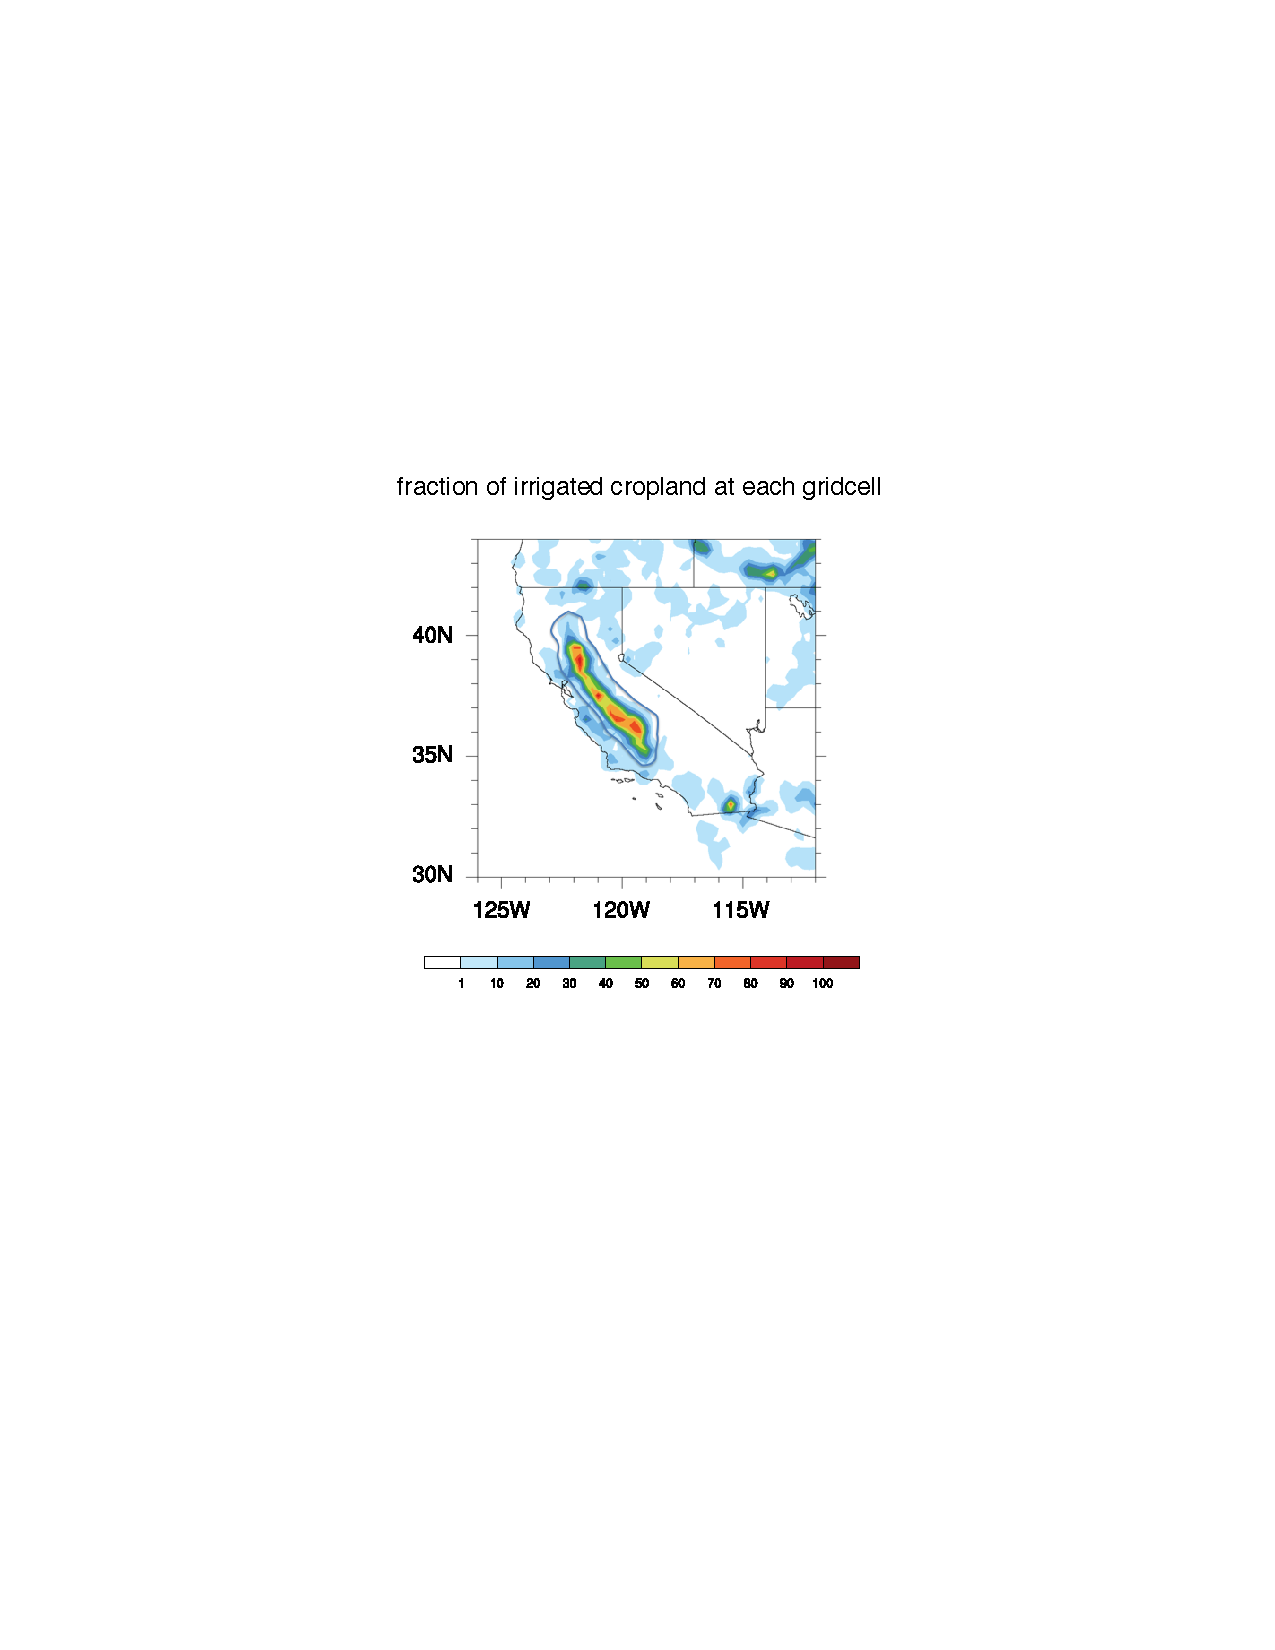
\includegraphics[width=6in]{irrigatedArea.pdf}
\caption{.}
\label{fig:Figure 1}
\end{center}
\end{figure}

\begin{figure}
\begin{center}
\includegraphics[width=6in]{irrig_2dplot_v2.pdf}
\caption{.}
\label{fig:Figure 1}
\end{center}
\end{figure}

\begin{figure}
\begin{center}
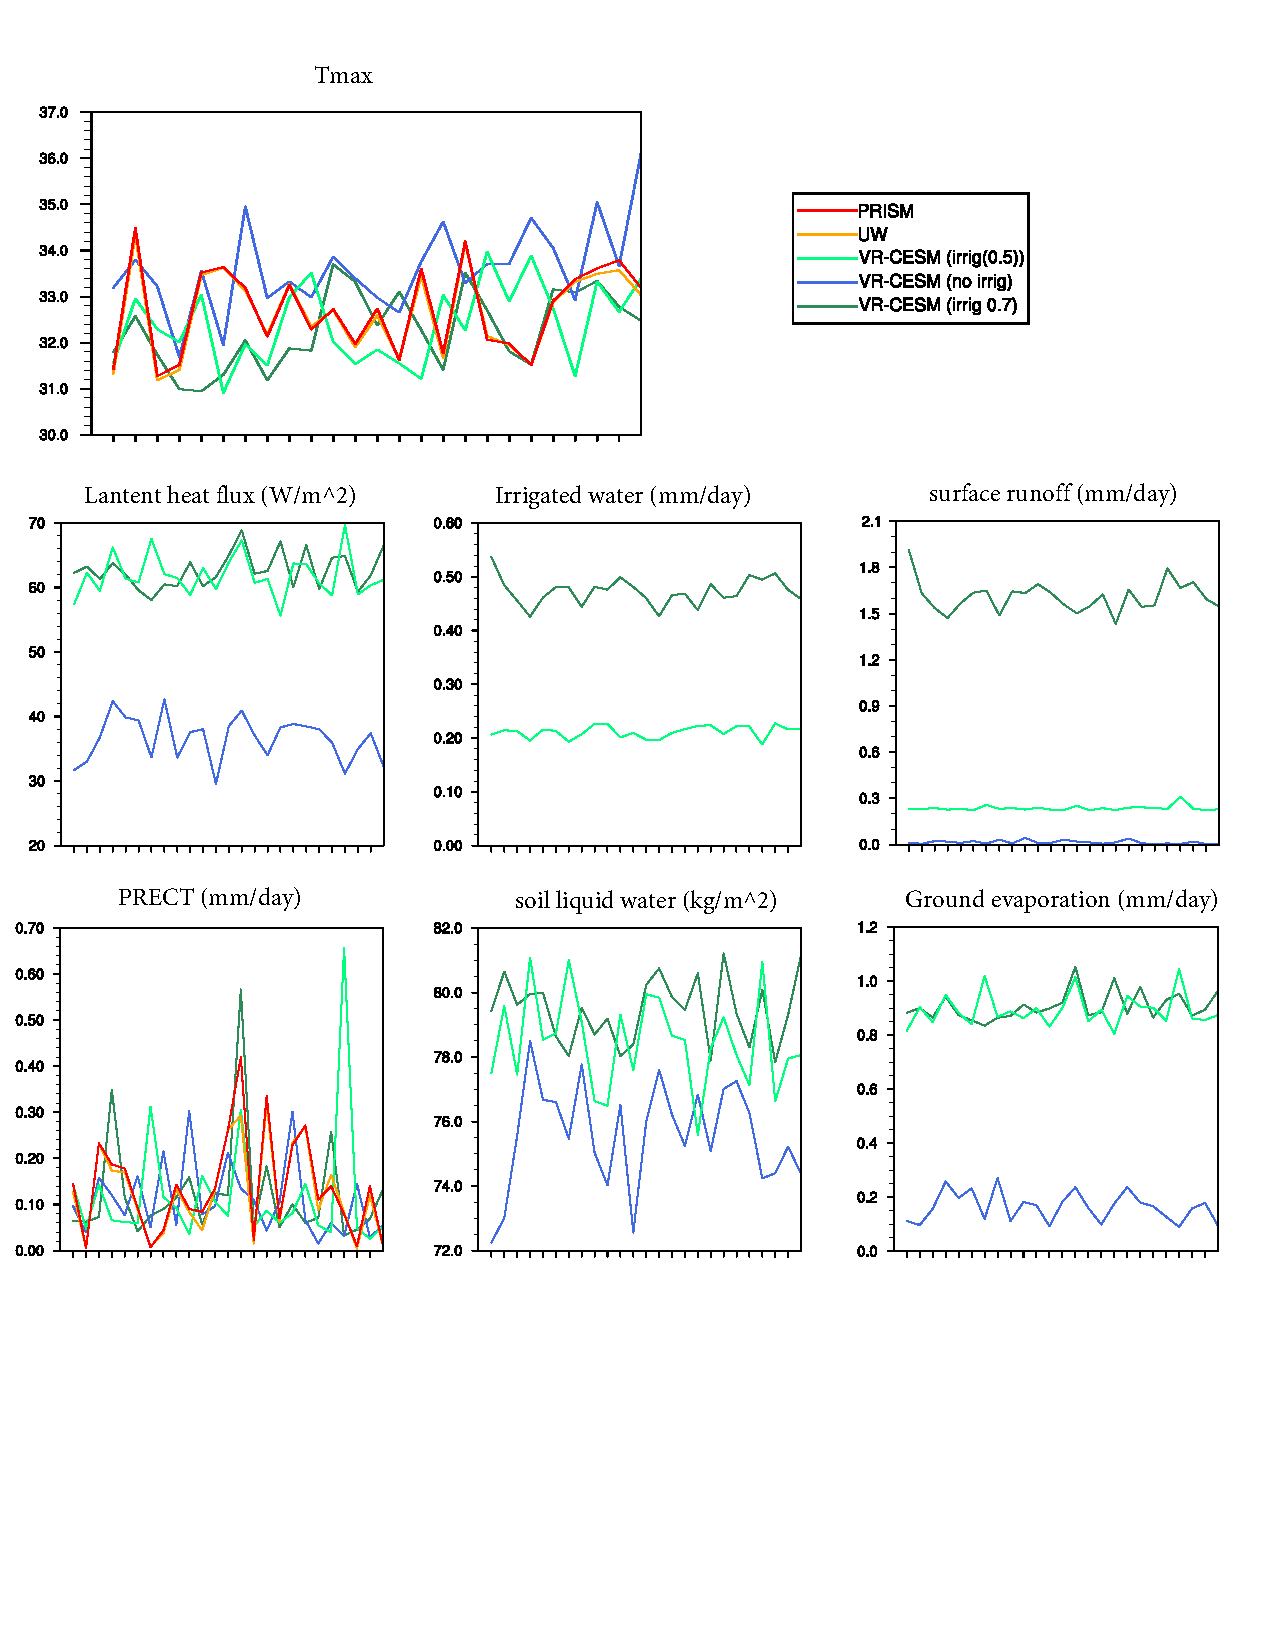
\includegraphics[width=6in]{irrig_trd_yearly_v2.pdf}
\caption{.}
\label{fig:Figure 3}
\end{center}
\end{figure}

\begin{figure}
\begin{center}
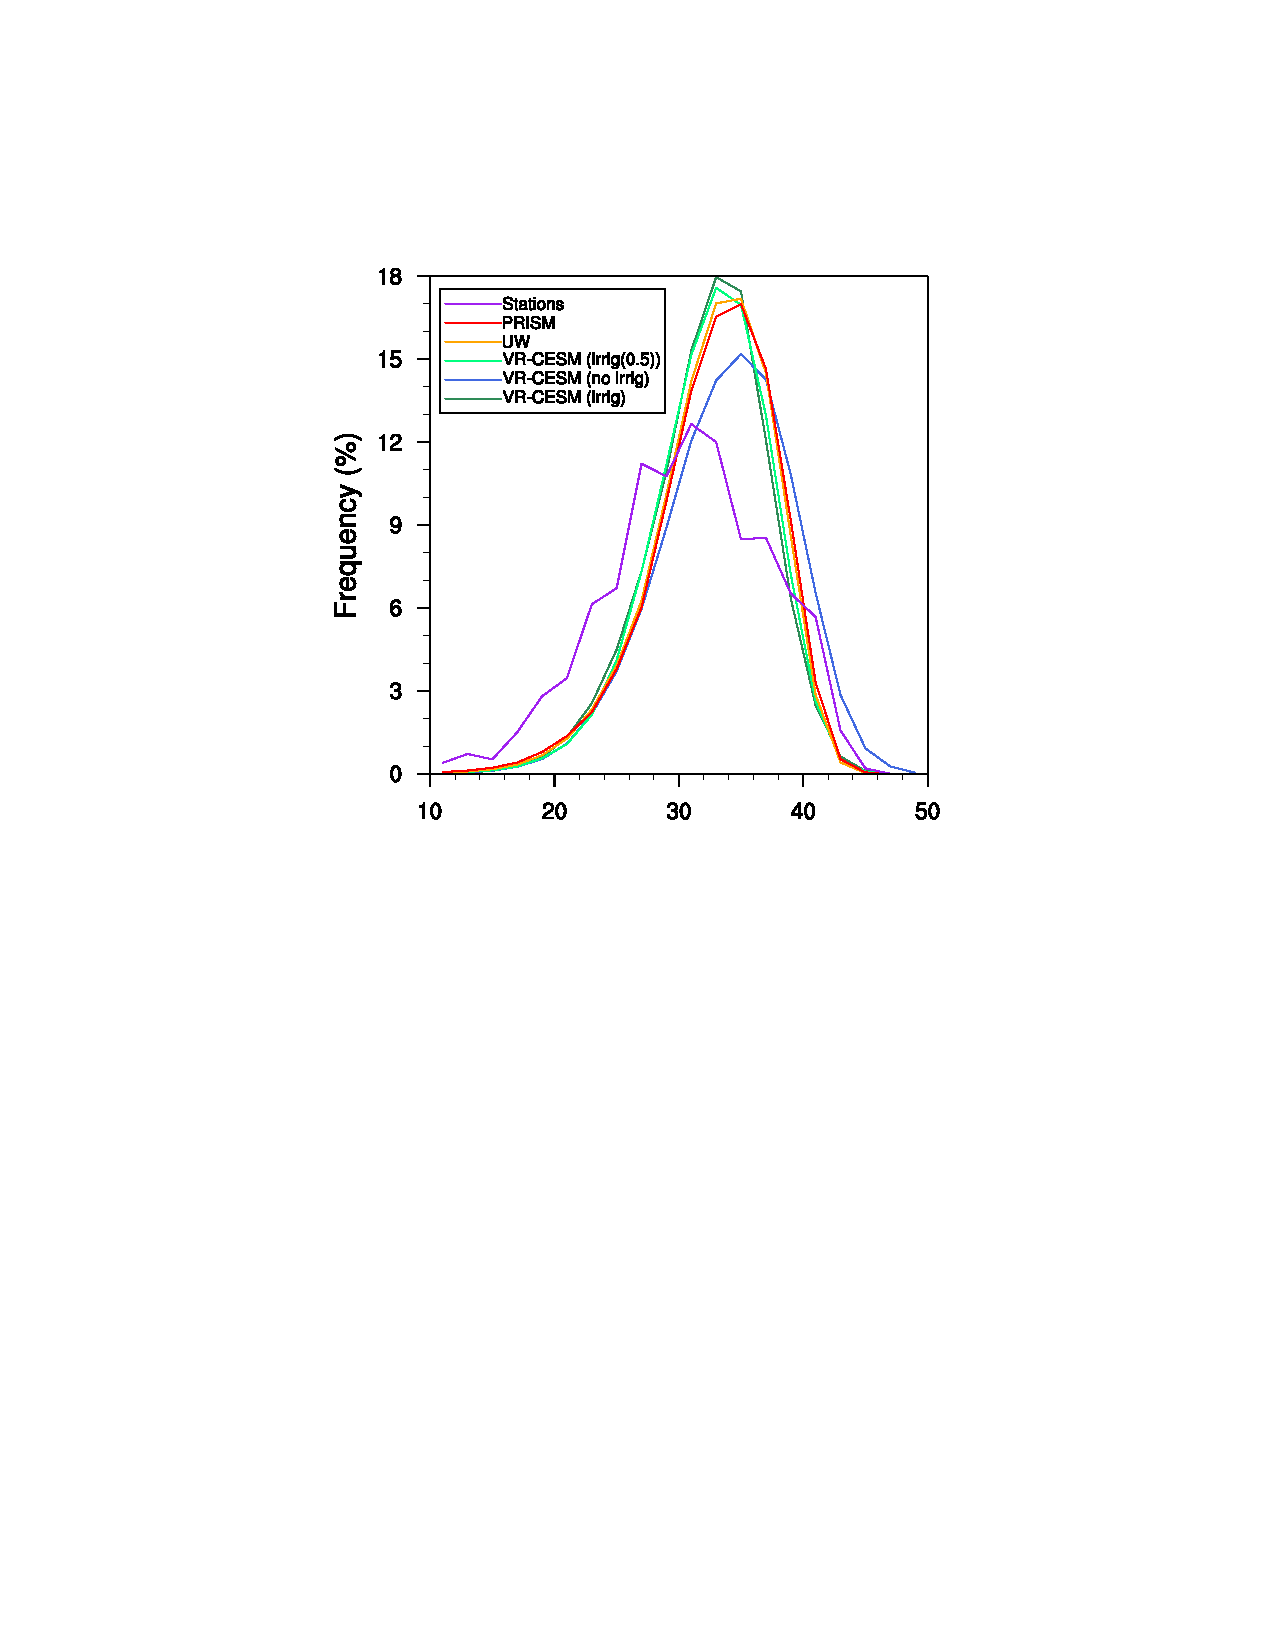
\includegraphics[width=6in]{irrig_pdf_v3.pdf}
\caption{.}
\label{fig:Figure 4}
\end{center}
\end{figure}

\begin{figure}
\begin{center}
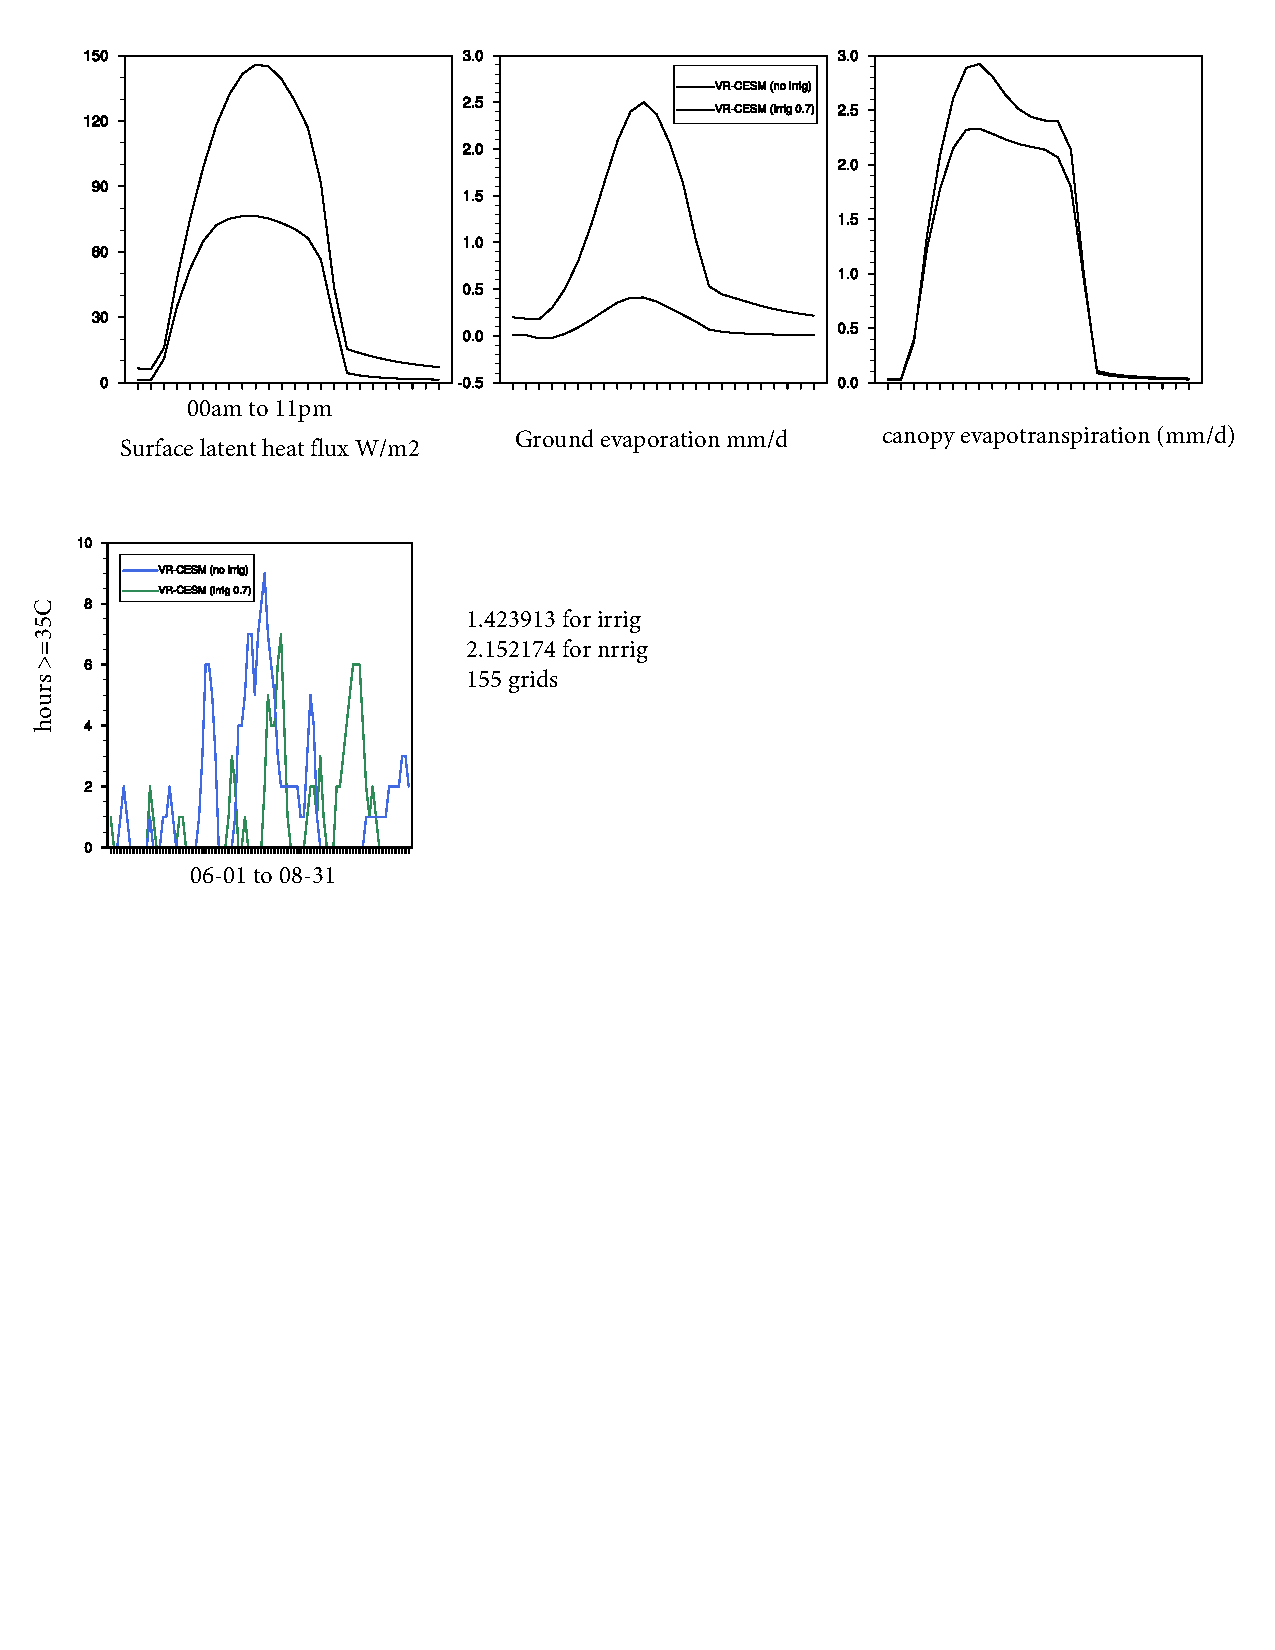
\includegraphics[width=6in]{irrig_trd_and_hours_T2>=35.pdf}
\caption{.}
\label{fig:Figure 5}
\end{center}
\end{figure}


\end{document}